\documentclass[t]{beamer}
\usetheme{Copenhagen}
\setbeamertemplate{headline}{} % remove toc from headers
\beamertemplatenavigationsymbolsempty

\usepackage{amsmath, array, tikz, bm, pgfplots, tcolorbox, tkz-euclide}
\usetkzobj{all}
\pgfplotsset{compat = 1.16}

\title{Distance and Midpoint in the Coordinate Plane}
\author{}
\date{}

% \begin{tcolorbox}[colframe=green!20!black, colback = green!30!white,title=\textbf{TITLE}]

\AtBeginSection[]
{
  \begin{frame}
    \frametitle{Objectives}
    \tableofcontents[currentsection]
  \end{frame}
}

\begin{document}

\begin{frame} 
\maketitle
\end{frame}

\section{Find the distance between two points in the coordinate plane}

\begin{frame}{Distance in the Coordinate Plane}
If we have points $A(x_1, y_1)$ and $B(x_2, y_2)$, then we can use the {\color{blue}\textbf{Pythagorean Theorem}} to find the distance between them.	\newline\\
\begin{minipage}{0.55\textwidth}
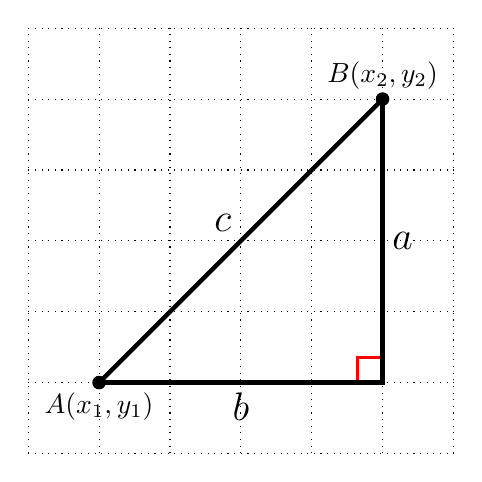
\begin{tikzpicture}[scale=0.9]
\draw[dotted] (-3,-3) grid (3,3);
\draw[fill] (-2,-2) circle [radius=2.5pt] node [below] {$A(x_1,y_1)$};
\draw[fill] (2,2) circle [radius=2.5pt] node [above] {$B(x_2,y_2)$};
\onslide<2->{\draw[color=red, very thick] (2,-2) rectangle +(-0.35,0.35);}
\draw[ultra thick] (-2,-2) -- (2,2);
\onslide<2->{\draw[ultra thick] (-2,-2) -- (2,-2) -- (2,2);}
\onslide<2->{\node at (0,-2) [below] {\Large $b$};}
\onslide<2->{\node at (2,0) [right] {\Large $a$};}
\onslide<2->{\node at (0,0) [above left] {\Large $c$};}
\end{tikzpicture}
\end{minipage}
\hspace{-0.5cm}
\begin{minipage}{0.40\textwidth}
\begin{align*}
\onslide<3->{c^2 &= a^2 + b^2} \\[10pt]
\onslide<4->{c &= \sqrt{a^2 + b^2}} \\[10pt]
\onslide<5->{&=\sqrt{(x_2-x_1)^2+(y_2-y_1)^2}}
\end{align*}
\end{minipage}
\end{frame}

\begin{frame}{Example 1}
Find the distance between each pair of points. Round your answers to 2 decimal places.	\newline\\
(a)	\quad $(5, \, 3)$ and $(-4, \, 7)$	\newline\\
\begin{minipage}{0.6\textwidth}
\onslide<2->{
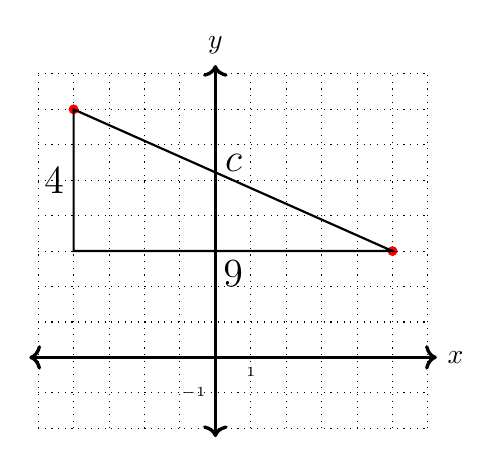
\begin{tikzpicture}[scale=0.45]
\coordinate (A) at (5,3);
\coordinate (B) at (-4,7);
\draw[dotted] (-5,-2) grid (6,8);
\draw[very thick, <->] (-5.25,0) -- (6.25,0) node [right] {$x$};
\draw[very thick, <->] (0,-2.25) -- (0,8.25) node [above] {$y$};
\draw[color=red,fill=red] (A) circle [radius=3.5pt];
\draw[color=red,fill=red] (B) circle [radius=3.5pt];
\node at (1,0) [below] {\tiny 1};
\node at (0,-1) [left] {\tiny $-1$};
\onslide<3->{\draw[thick] (A) -- (B) -- (-4,3) -- cycle;}
\onslide<4->{\node at (-4,5) [left] {\Large 4};}
\onslide<5->{\node at (0.5,3) [below] {\Large 9};}
\onslide<6->{\node at (0,5.5) [right] {\Large $c$};}
\end{tikzpicture}}
\end{minipage}
\begin{minipage}{0.3\textwidth}
\begin{align*}
\onslide<7->{c^2 &= 4^2 + 9^2} \\
\onslide<8->{c^2 &= 16 + 81} \\
\onslide<9->{c^2 &= 95} \\
\onslide<10->{c &= \sqrt{95}} \\
\onslide<11->{c &\approx 9.75}
\end{align*}
\end{minipage}
\end{frame}

\begin{frame}{Example 1}
(b)	\quad $(0, \, -6)$ and $(3, \, -1)$	\newline\\
\begin{minipage}{0.6\textwidth}
\onslide<2->{
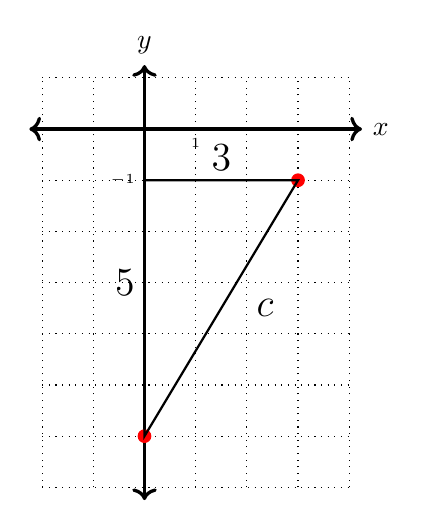
\begin{tikzpicture}[scale=0.65]
\coordinate (A) at (0,-6);
\coordinate (B) at (3,-1);
\draw[dotted] (-2,-7) grid (4,1);
\draw[very thick, <->] (-2.25,0) -- (4.25,0) node [right] {$x$};
\draw[very thick, <->] (0,-7.25) -- (0,1.25) node [above] {$y$};
\draw[color=red,fill=red] (A) circle [radius=3.5pt];
\draw[color=red,fill=red] (B) circle [radius=3.5pt];
\node at (1,0) [below] {\tiny 1};
\node at (0,-1) [left] {\tiny $-1$};
\onslide<3->{\draw[thick] (A) -- (B) -- (0,-1) -- cycle;}
\onslide<4->{\node at (0,-3) [left] {\Large 5};}
\onslide<5->{\node at (1.5,-1) [above] {\Large 3};}
\onslide<6->{\node at (2,-3.5) [right] {\Large $c$};}
\end{tikzpicture}}
\end{minipage}
\begin{minipage}{0.3\textwidth}
\begin{align*}
\onslide<7->{c^2 &= 3^2 + 5^2} \\
\onslide<8->{c^2 &= 9 + 25} \\
\onslide<9->{c^2 &= 34} \\
\onslide<10->{c &= \sqrt{34}} \\
\onslide<11->{c &\approx 5.83}
\end{align*}
\end{minipage}
\end{frame}


\begin{frame}{Example 1}
(c)	\quad $(1, \, 8)$ and $(-5, \, 8)$	\newline\\
\begin{minipage}{0.6\textwidth}
\onslide<2->{
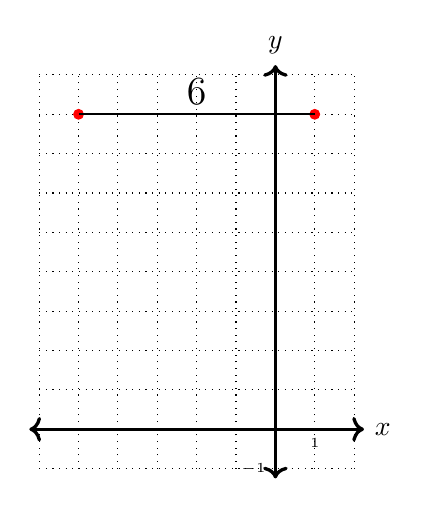
\begin{tikzpicture}[scale=0.5]
\coordinate (A) at (1,8);
\coordinate (B) at (-5,8);
\draw[dotted] (-6,-1) grid (2,9);
\draw[very thick, <->] (-6.25,0) -- (2.25,0) node [right] {$x$};
\draw[very thick, <->] (0,-1.25) -- (0,9.25) node [above] {$y$};
\draw[color=red,fill=red] (A) circle [radius=3.5pt];
\draw[color=red,fill=red] (B) circle [radius=3.5pt];
\node at (1,0) [below] {\tiny 1};
\node at (0,-1) [left] {\tiny $-1$};
\onslide<3->{\draw[thick] (A) -- (B);}
\onslide<4->{\node at (-2,8) [above] {\Large 6};}
\end{tikzpicture}}
\end{minipage}
\end{frame}

\section{Find the midpoint between two points in the coordinate plane}

\begin{frame}{Midpoint}
The {\color{blue}\textbf{midpoint}} between 2 points in the coordinate plane is the mean average of the $x$-coordinates and the mean average of the $y$-coordinates.	\newline\\
\begin{center}
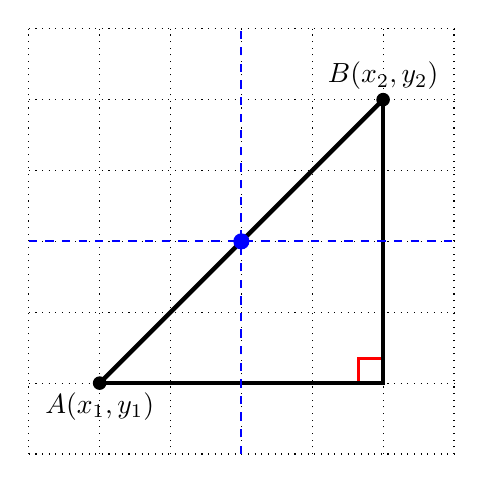
\begin{tikzpicture}[scale=0.9]
\draw[dotted] (-3,-3) grid (3,3);
\draw[fill] (-2,-2) circle [radius=2.5pt] node [below] {$A(x_1,y_1)$};
\draw[fill] (2,2) circle [radius=2.5pt] node [above] {$B(x_2,y_2)$};
\onslide<2->{\draw[color=red, very thick] (2,-2) rectangle +(-0.35,0.35);}
\draw[ultra thick] (-2,-2) -- (2,2);
\onslide<2->{\draw[ultra thick] (-2,-2) -- (2,-2) -- (2,2);}
\onslide<3->{\draw[dashed,color=blue,thick] (0,-3) -- (0,3);}
\onslide<4->{\draw[dashed,color=blue,thick] (-3,0) -- (3,0);}
\onslide<5->{\draw[color=blue,fill=blue] (0,0) circle [radius=3pt];}
\end{tikzpicture}
\end{center}
\end{frame}

\begin{frame}{Midpoint}
The {\color{blue}\textbf{midpoint}} between 2 points in the coordinate plane is the mean average of the $x$-coordinates and the mean average of the $y$-coordinates.	\newline\\
\begin{center}
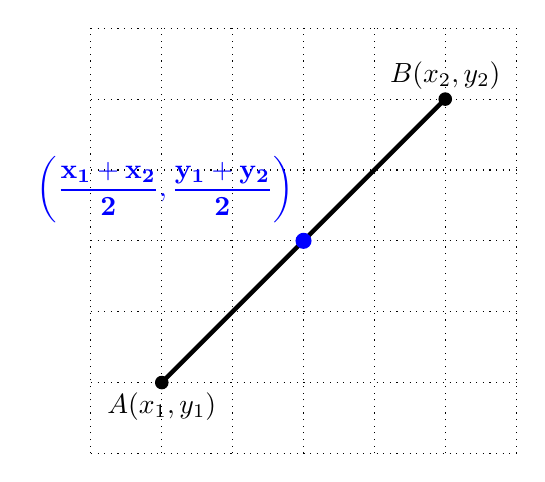
\begin{tikzpicture}[scale=0.9]
\draw[dotted] (-3,-3) grid (3,3);
\draw[fill] (-2,-2) circle [radius=2.5pt] node [below] {$A(x_1,y_1)$};
\draw[fill] (2,2) circle [radius=2.5pt] node [above] {$B(x_2,y_2)$};
\draw[ultra thick] (-2,-2) -- (2,2);
\draw[color=blue,fill=blue] (0,0) circle [radius=3pt];
\node at (0,0) [above left,color=blue,yshift=0.1cm] {$\mathbf{\left(\dfrac{x_1+x_2}{2},\dfrac{y_1+y_2}{2}\right)}$};
\end{tikzpicture}
\end{center}
\end{frame}

\begin{frame}{Example 2}
Find the midpoint of each pair of points.	\newline\\
(a)	\quad $A(4, \, -7) \text{ and } B(9, \, -4)$	\newline\\
\onslide<2->{Average of $x$-coordinates:}
\onslide<3->{\[\frac{4+9}{2} = \frac{13}{2}\]}
\onslide<4->{Average of $y$-coordinates:}
\onslide<5->{\[\frac{-7+(-4)}{2} = -\frac{11}{2}\]}
\onslide<6->{Midpoint: $\left(\dfrac{13}{2}, -\dfrac{11}{2}\right)$}
\end{frame}

\begin{frame}{Example 2a}
\begin{center}
\begin{tikzpicture}
\coordinate (A) at (4,-7);
\coordinate (B) at (9,-4);
\coordinate (M) at (6.5,-5.5);
\draw[dotted] (3,-8) grid (10,-3);
\draw[color=red,fill=red] (A) circle [radius=3pt];
\draw[color=red,fill=red] (B) circle [radius=3pt];
\draw[thick] (A) -- (B);
\draw[color=blue,fill=blue] (M) circle [radius=3pt];
\onslide<2->{
\draw[thick,dashed] (A) -- (6.5,-7) -- (M) -- (9,-5.5) -- (B);
\onslide<3->{
\node at (5.25,-7) [below] {2.5};
\node at (6.5,-6.25) [right] {1.5};
\node at (8,-5.5) [below] {2.5};
\node at (9,-4.75) [right] {1.5};}}
\end{tikzpicture}
\end{center}
\end{frame}

\begin{frame}{Example 2}
(b)	\quad	$(-9, \, 1)$ and $(-9, \, 4)$	\newline\\
\onslide<2->{Average of $x$-coordinates:}
\onslide<3->{\[\frac{-9+(-9)}{2} = -9\]}
\onslide<4->{Average of $y$-coordinates:}
\onslide<5->{\[\frac{1+4}{2} = \frac{5}{2}\]}
\onslide<6->{Midpoint: $\left(-9, \dfrac{5}{2}\right)$}
\end{frame}

\begin{frame}{Example 2b}
\begin{center}
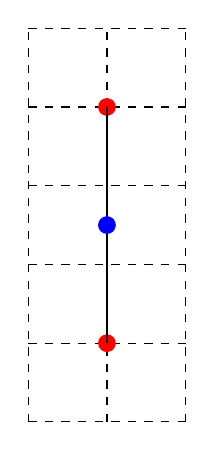
\begin{tikzpicture}
\coordinate (A) at (-9,1);
\coordinate (B) at (-9,4);
\draw[dashed] (-10, 0) grid (-8,5);
\draw[color=red,fill=red] (A) circle [radius=3pt];
\draw[color=red,fill=red] (B) circle [radius=3pt];
\draw[thick] (A) -- (B);
\onslide<2->{\draw[color=blue,fill=blue] (-9,2.5) circle [radius=3pt];}
\end{tikzpicture}
\end{center}
\end{frame}

\begin{frame}{Example 3}
Find the coordinates of $B$ if $M$ is the midpoint of $\overline{AB}$.	\newline\\
(a)	\quad	$A(-10, \, -1)$;  $M(-4, \, 0)$	\newline\\
\onslide<2->{
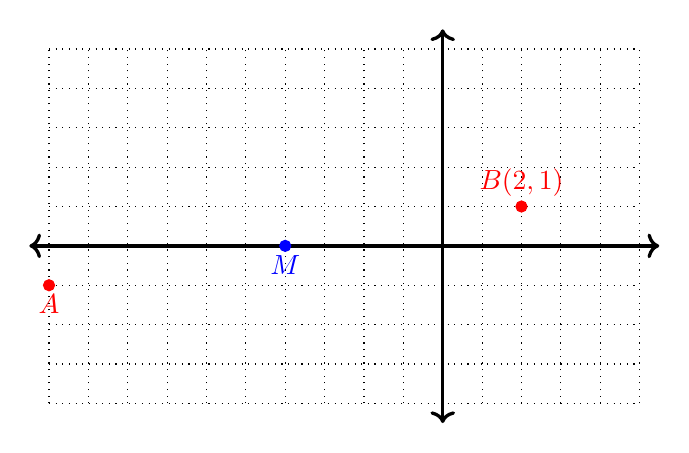
\begin{tikzpicture}[scale=0.5]
\coordinate (A) at (-10,-1);
\coordinate (M) at (-4,0);
\draw[dotted] (-10,-4) grid (5,5);
\draw[very thick, <->] (-10.5,0) -- (5.5,0);
\draw[very thick, <->] (0,-4.5) -- (0,5.5);
\draw[color=red,fill=red] (A) circle [radius=4pt] node [below] {$A$};
\draw[color=blue,fill=blue] (M) circle [radius=4pt] node [below] {$M$};
\onslide<3->{\draw[color=red,fill=red] (2,1) circle [radius=4pt];}
\onslide<4->{\node at (2,1) [above,color=red] {$B(2,1)$};}
\end{tikzpicture}}
\end{frame}

\begin{frame}{Example 3}
(b)	\quad	$A(6, \, -4)$;  $M(3, \, 3)$	\newline\\
\onslide<2->{
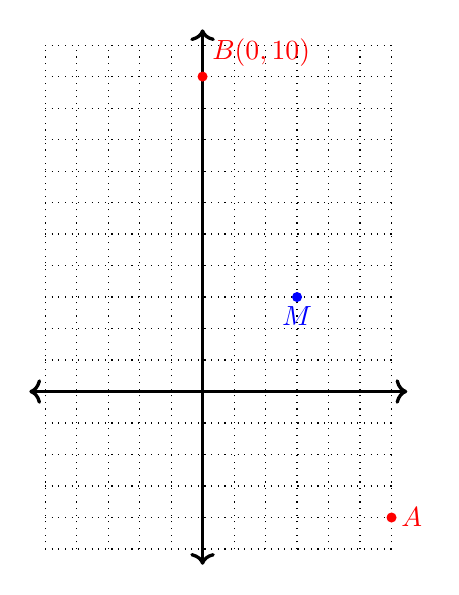
\begin{tikzpicture}[scale=0.4]
\coordinate (A) at (6,-4);
\coordinate (M) at (3,3);
\draw[dotted] (-5,-5) grid (6,11);
\draw[very thick, <->] (-5.5,0) -- (6.5,0);
\draw[very thick, <->] (0,-5.5) -- (0,11.5);
\draw[color=red,fill=red] (A) circle [radius=4pt] node [right] {$A$};
\draw[color=blue,fill=blue] (M) circle [radius=4pt] node [below] {$M$};
\onslide<3->{\draw[color=red,fill=red] (0,10) circle [radius=4pt];}
\onslide<4->{\node at (0,10) [above right,color=red] {$B(0,10)$};}
\end{tikzpicture}}
\end{frame}


\end{document}